% 第7章 評価
\newpage
\renewcommand{\baselinestretch}{1.5}
\section{評価}\label{sec:evaluation}
\renewcommand{\baselinestretch}{1}
\par 本手法を評価する為に要素の顕著度推定の精度に関する評価とウェブページの顕著性マップの可視化を目的として提案した顕著領域マップならびに集約図の認識のしやすさと効果に関する3つの実験を実施した。

\subsection{評価方法}
\subsubsection{要素の顕著度推定精度に関する評価}
\par 1つ目の評価では本手法の特徴であるウェブページの要素の顕著度推定精度を測る。第\ref{subsec:webdataset}節で作成したオリジナルのウェブデータセットをランダムに4:1の割合で分析用のページ216個と評価用のページ54個に分類したが、その54個の評価用ウェブページとその実際の被験者視線データを使用して評価を行う。実験の評価指標としてBylinskiiらの公開プログラム\cite{salMetrics_Bylinskii}のArea Under the Curve (AUC), Linear Correlation Coefficient (CC)とKullback\-Leibler divergence (KL)の3つの顕著性メトリクスを使用した。

\par {\bf AUC (Area Under the Curve)}は顕著性マップ生成モデルに最もよく使用されるメトリクスで横軸を注視点の誤検出率、縦軸を注視点の検出率としたROC曲線の曲線下の面積を計測する評価指標である。$0\sim1$の間で評価され、$0.5$の時にランダムであることを表し$1$に近いほど精度の高い顕著性マップであることを示す。{\bf CC (Linear Correlation Coefficient)}はオリジナルモデルの顕著性マップと実際の被験者の視線データから作成された基準顕著性マップの間の相関係数を計測する評価指標である。CCは$-1\sim1$の間で評価され、$1$に近いほど精度の高い顕著性マップであることを示す。{\bf KL (Kullback\-Leibler divergence)}はオリジナルモデルの顕著性マップと基準顕著性マップの2つの確率分布がどの程度似ているのかを計測する評価指標である。KLは今まで説明した2つのメトリクスとは異なり、2つのマップが同じ確率分布である場合に$0$と評価される為、$0\sim1$の間で評価され、$0$に近いほど精度の高い顕著性マップであることを示す。

\par 評価実験では54個の評価用ウェブページを使用して基準顕著領域マップと本研究のオリジナルモデルとプログラムが公開されている関連研究を比較した。評価を行う為に第\ref{subsec:gazedataset}節で取得した被験者の実際の視線データを使用して第\ref{subsec:system04-1}項で説明した手法で基準顕著領域マップを作成した。また、関連研究として公開されている中で評価が高い自然画像向けニューラルネットワーク顕著性マップ生成モデルであるPanらのSalNet\cite{pan2016shallow}とCorniaらのML-NET\cite{mlnet2016}を使用した。さらにオリジナルモデルではIttiらのベーシックな顕著性マップ生成モデル\cite{itti1998model}を使用しているが、顕著性マップ生成モデルを変更することでオリジナルモデルにCorniaらのML-NET\cite{mlnet2016}を組み合わせたものも比較モデルに加える。


\subsubsection{重要領域の認識のしやすさに関する評価}
\par 2つ目の評価方法では最もベーシックなモデルであるIttiらの顕著性マップ生成モデル\cite{itti1998model}と提案手法の顕著領域マップでの重要領域の認識のしやすさについて比較評価した。本実験では20代の19$\sim$25歳の大学生・大学院生10人の日常的にインターネットを使用するインターネットユーザーに対してインタビュー形式で実験を行った。

\par 評価では被験者に顕著性マップの概要について簡単に説明した後に既存の顕著性マップと提案手法の顕著領域マップの例を2つ提示して最後に全7問の表\ref{table:question01}に示す内容のアンケートを実施した。アンケートでは既存の顕著性マップと提案手法の顕著領域マップの重要領域の認識のしやすさの度合いと、どのような点で認識しやすく感じたり認識しにくいと感じるのかを記述式で質問した。また、実験にはJapan Web Design Gallery\cite{japanwebgallery}に掲載されているウェブページの中からランダムに選んだ2つのウェブページ情報を使用した。実験に使用したウェブページの一覧を表\ref{table:webpage-list2}に示す。また、実際に被験者に見せたウェブページと顕著性マップと顕著領域マップの比較を図\ref{fig_experience02}に示す。


\begin{table}[h]
  \caption{重要領域認識実験に使用したウェブページの一覧(2019年1月20日閲覧)}
  \label{table:webpage-list2}
  \centering
  \begingroup
  \renewcommand{\arraystretch}{1.2} % 表の行間の変更
  \small
    \begin{tabular}{lll}
    \hline
    ページ名 & カテゴリ & URL \\
    \hline \hline
    下関春帆楼 & カフェ・レストラン & https://www.shunpanro.com/ \\
    白洋舎 & クリーニング & http://www.hakuyosha.co.jp/ \\
    \hline
  \end{tabular}
  \endgroup
\end{table}

\begin{figure}[H]
  \centering
  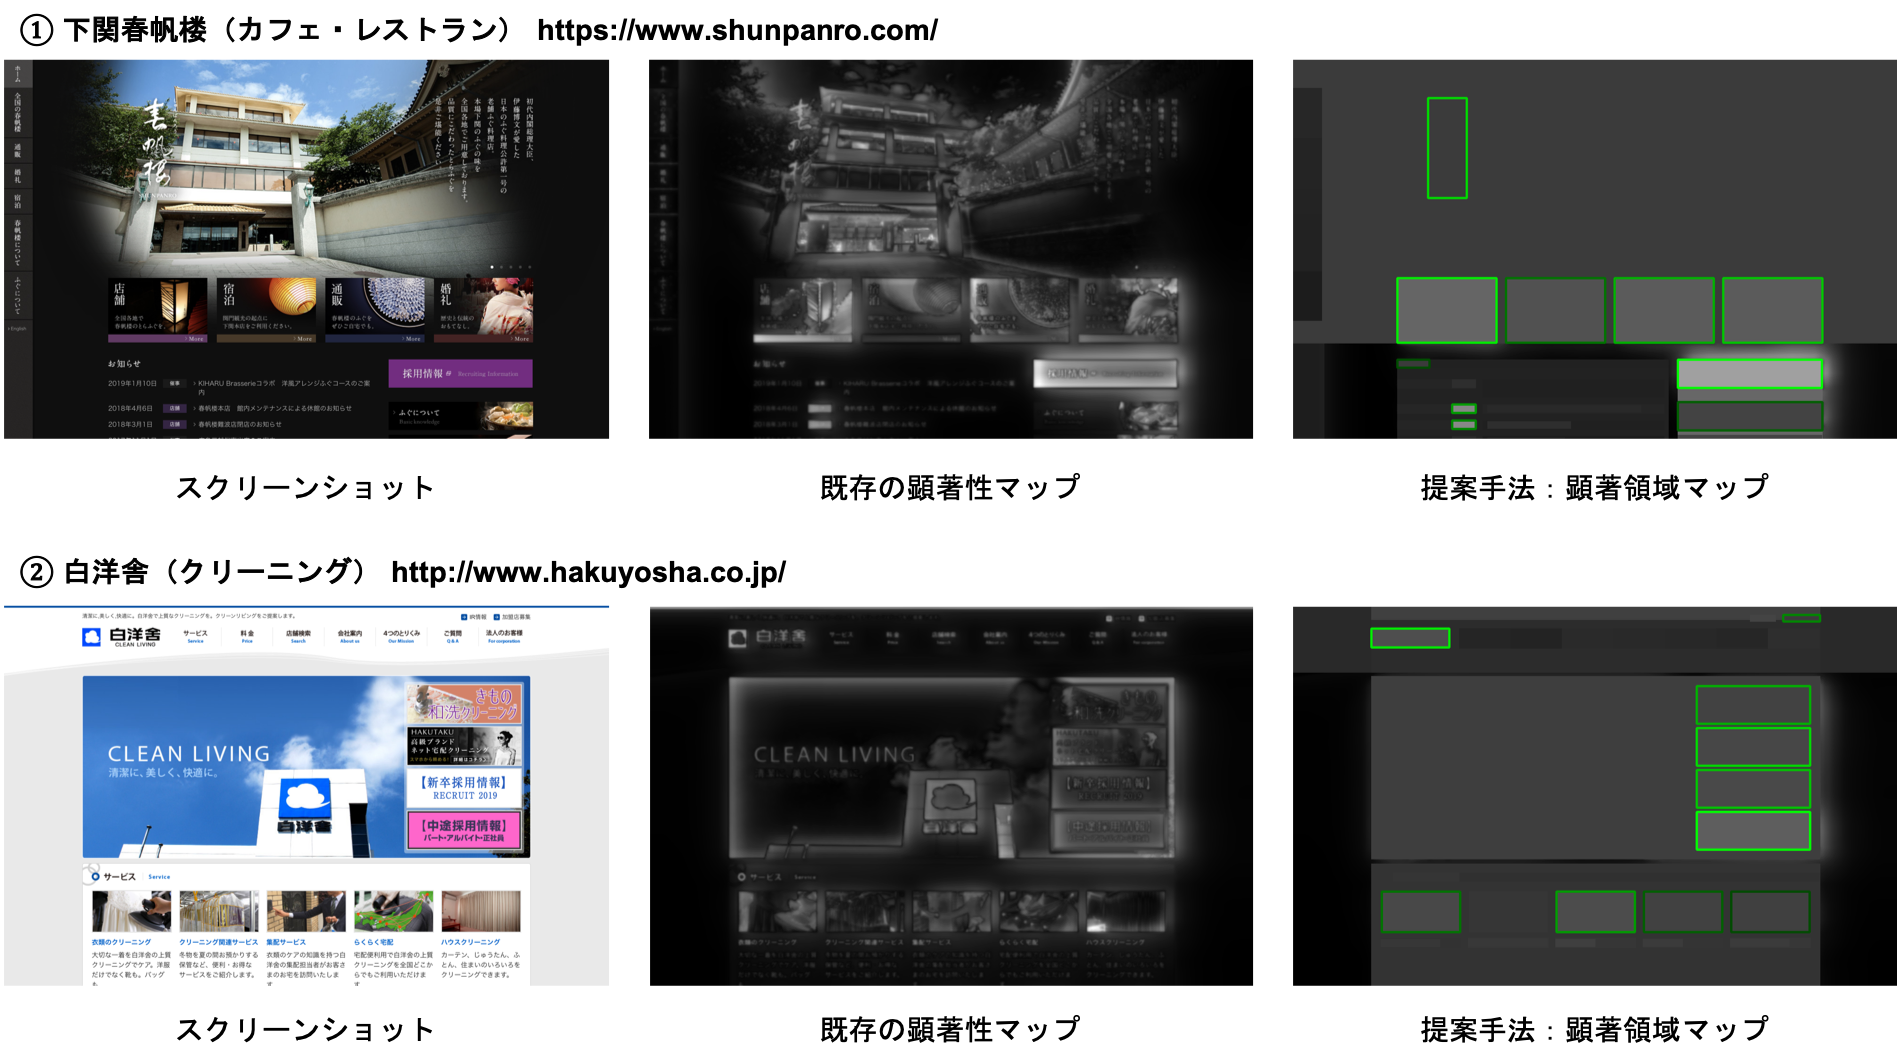
\includegraphics[width=12cm]{figures/07_experience02.png}
  \caption{既存の顕著性マップと提案手法(顕著領域マップ)の比較実験}
  \label{fig_experience02}
\end{figure}

\begin{table}[h]
  \caption{アンケートの質問内容1}
  \label{table:question01}
  \centering
  \begingroup
  \renewcommand{\arraystretch}{1} % 表の行間の変更
  \small
  \begin{tabular}{|l|l|l|l|}
    \hline
    \multicolumn{2}{|c|}{質問内容} & \multicolumn{2}{|c|}{選択肢・記述式} \\ \hline
    & & a & 非常に認識しにくい \\ \cline{3-4}
    & & b & 認識しにくい \\ \cline{3-4}
    Q1 & 既存の顕著性マップは & c & どちらでもない \\ \cline{3-4}
    & 重要領域を認識しやすいと感じるか & d & 認識しやすい \\ \cline{3-4}
    & & e & 非常に認識しやすい \\ \hline
    & & a & 非常に認識しにくい \\ \cline{3-4}
    & & b & 認識しにくい \\ \cline{3-4}
    Q2 & 提案手法の顕著領域マップは & c & どちらでもない \\ \cline{3-4}
    & 重要領域を認識しやすいと感じるか & d & 認識しやすい \\ \cline{3-4}
    & & e & 非常に認識しやすい \\ \hline
    Q3 & 既存の顕著性マップの認識しづらいと感じる点 & \multicolumn{2}{|l|}{記述式} \\ \hline
    Q4 & 既存の顕著性マップの認識しやすいと感じる点 & \multicolumn{2}{|l|}{記述式} \\ \hline
    Q5 & 顕著領域マップの認識しづらいと感じる点 & \multicolumn{2}{|l|}{記述式} \\ \hline
    Q6 & 顕著領域マップの認識しやすいと感じる点 & \multicolumn{2}{|l|}{記述式} \\ \hline
    Q7 & 特定の要素の重要度を調べたい時 & a & 既存の手法 \\ \cline{3-4}
    & どちらの手法が認識しやすいと感じるか  & b & 提案手法 \\ \hline
    \end{tabular}
    \endgroup
\end{table}


\subsubsection{集約図の効果に関する評価}
\par 3つ目の評価方法では特に顕著度が高い重要領域をタイル状に並べてまとめた集約図の効果について評価した。本実験についても20代の19$\sim$25歳の大学生・大学院生10人の日常的にインターネットを使用するインターネットユーザーに対してインタビュー形式で実験を行った。

\par 評価ではまず始めに被験者に図\ref{fig_experience03-2}に示す集約図の例を見せ集約図の意味について簡単に説明したのちに、図\ref{fig_experience03-1}に示す集約図を見てウェブページの内容を予想してもらい、分かる範囲でページ内容を記述式で回答してもらった。また、ウェブページの予測をしてもらった後に表\ref{table:question02}に示す集約図の効果に関する2問の質問に選択式で解答してもらった。なお、アンケートの最後には自由記入形式の感想欄を設けて集約図をみた際の感想などを記述してもらった。集約図の効果検証実験に使用したウェブページを表\ref{table:webpage-list3}に示す。

\begin{table}[h]
    \caption{集約図の効果評価実験に使用したウェブページ(全て2019年1月20日閲覧)}
    \label{table:webpage-list3}
    \centering
    \begingroup
    \renewcommand{\arraystretch}{1.2} % 表の行間の変更
    \small
      \begin{tabular}{lll}
      \hline
      ページ名 & カテゴリ & URL \\
      \hline \hline
      株式会社エース & コンビニ・スーパー・小売り & https://www.ace-group.co.jp/ \\
      \hline
    \end{tabular}
    \endgroup
\end{table}

\begin{figure}[H]
    \centering
    
\includegraphics[width=10cm]{figures/experience03-2.png}
    \caption{被験者に閲覧してもらった集約図の例}
    \label{fig_experience03-2}
\end{figure}

\begin{figure}[H]
    \centering
    
\includegraphics[width=6cm]{figures/experience03-1.png}
    \caption{ページ内容を予想してもらった集約図(株式会社エースHP)}
    \label{fig_experience03-1}
\end{figure}

\begin{table}[H]
    \caption{アンケートの質問内容2}
    \label{table:question02}
    \centering
    \begingroup
    \renewcommand{\arraystretch}{1} % 表の行間の変更
    \small
    \begin{tabular}{|l|l|l|l|}
        \hline
        \multicolumn{2}{|c|}{質問内容} & \multicolumn{2}{|c|}{選択肢} \\ \hline
        & & a & 全く判断できない \\ \cline{3-4}
        Q8 & 重要領域のみを抽出した集約図を見て & b & 少し判断できる \\ \cline{3-4}
        & ページ内容を判断することはできるか & c & ある程度判断できる \\ \cline{3-4}
        & & d & ほとんど判断できる \\ \hline
        & & a & 全く効果的でない \\ \cline{3-4}
        & 初見のウェブページの内容を一目で & b & あまり効果的でない \\ \cline{3-4}
        Q9 & 確認したい時重要領域を抽出してまとめる & c & どちらでもない \\ \cline{3-4}
        & 手法は効果的だと思うか & d & 効果的である \\ \cline{3-4}
        & & e & 非常に効果的である \\ \hline
        \end{tabular}
        \endgroup
\end{table}

\newpage
\subsection{結果と考察}
\subsubsection{要素の顕著度推定精度に関する評価}\label{subsec:evaluation1}
\par 1つ目の評価方法では被験者の実際の視線から作成した基準顕著領域マップと本手法の顕著領域マップとML-NETを組み合わせたモデルならびに2つの顕著性マップ生成モデルをCCとAUCとKLの3つのメトリクスで評価を行った。なお、基準顕著領域マップと比較対象のモデルについては各モデルのピクセルレベルの顕著性マップを第\ref{subsec:system04-1}節で説明した手順で要素単位の顕著領域マップに変換した上でオリジナルモデルと比較実験を行った。ウェブページデータセットの評価用データ54個の中からいくつか選んでそれぞれのモデルを比較した様子を図\ref{fig_07_eval-models}に示す。基準顕著性マップは1つのウェブページあたり5名の被験者の全ての視線データを加算して作成された実際の顕著性マップで被験者が閲覧した領域を正確に表している。また、基準顕著性マップを元に要素単位の顕著度を計算して各要素を顕著度に応じた明度で塗り潰したものが基準顕著領域マップである。この基準顕著領域マップとオリジナルモデルや比較モデルであるML-NETやSalNetの類似度を検証することで各モデルの精度を計算した。

\par 図\ref{fig_07_eval-models}を見ると各モデルによって顕著領域マップの出力が大きく異なることが確認できる。各ウェブページの要素の明度は顕著度を表しており、明るい要素ほど注目されやすいことを示し暗い要素ほど注目されにくい要素であることを示す。ウェブページによって基準データに近いモデルは異なるが他のモデルと比較して本手法のオリジナルモデルは基準顕著領域マップに近いことが確認できる。

\par 評価用の合計54個全てのウェブページの比較検証を行い各メトリクスの平均を計算した結果を表\ref{table:model-perfomance}に示す。調査の結果より3個のメトリクスの内、顕著性マップ生成モデルの評価指標として最もよく使われるAUCとKLの2つのメトリクスではオリジナルモデルが最も良いスコアを獲得した。また、CCについてもオリジナルモデルはML-NETに劣るスコアになったものの、オリジナルモデルにML-NETを組み合わせたモデルが最も良いスコアを獲得した。メトリクスの一つであるCCで他のモデルに劣るスコアが計測されたことはCC(Linear Correlation Coefficient)はマップの間の相関係数を計測する評価指標であるため画像間の輝度の差を計算することが原因であると考えられる。隣り合う各要素の顕著度のバランスの精度が高くても全体的に顕著度が低く出力されることで結果的に相関係数が低くなってしまったと考える。しかしながら、全体的にオリジナルモデルは要素の顕著度推定精度は高くウェブページの顕著領域マップを生成するモデルとして最適であると言える。


\begin{figure}[H]
  \centering
  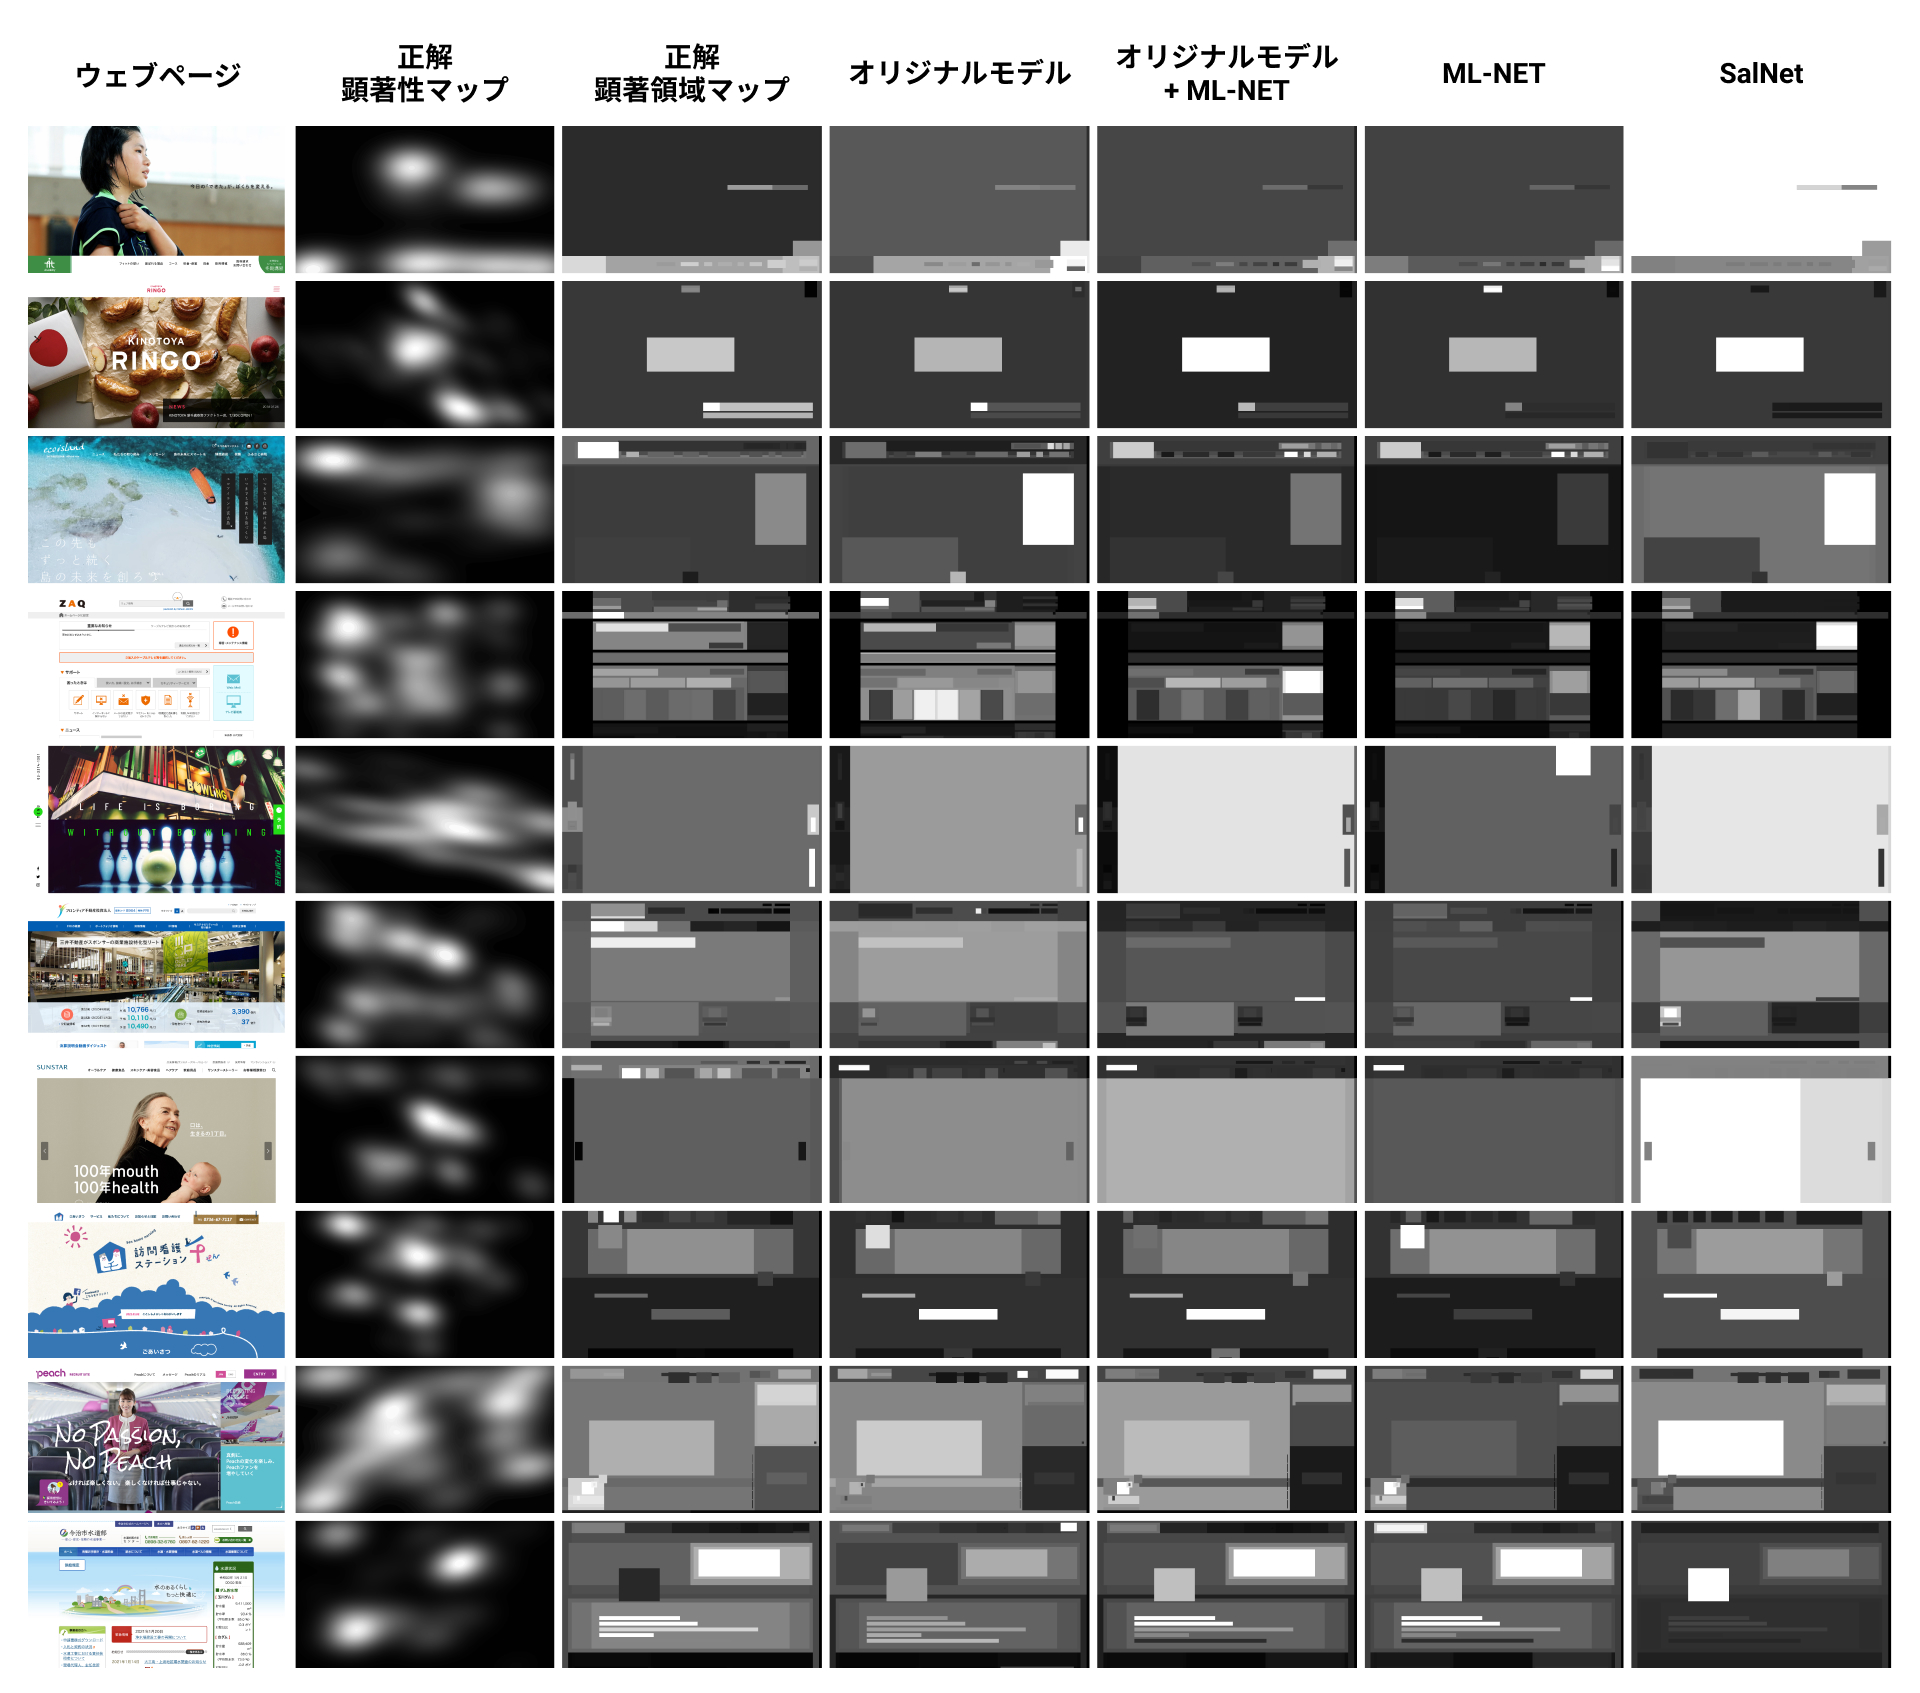
\includegraphics[width=12.5cm]{figures/07_eval-models.jpg}
  \caption{オリジナルモデルと顕著性マップモデルの比較}
  \label{fig_07_eval-models}
\end{figure}

\begin{table}[h]
  \caption{異なるモデル間でのパフォーマンス評価}
  \label{table:model-perfomance}
  \centering
  \begingroup
  \renewcommand{\arraystretch}{1.2} % 表の行間の変更
  \small
   \begin{tabular}{lccc}
    \hline
    & AUC↑ & CC↑ & KL↓ \\
    \hline \hline
    オリジナル & {\bf 0.78612} & 0.53475 & {\bf 0.12348} \\
    オリジナル + ML-NET & 0.74319 & {\bf 0.55167} & 0.13691 \\
    SalNet & 0.66270 & 0.36863 & 0.14679 \\
    ML-NET & 0.74279 & 0.54798 & 0.13777 \\
    \hline
  \end{tabular}
  \endgroup
\end{table}


\subsubsection{重要領域の認識のしやすさに関する評価}
\par 2つ目の評価方法では既存の顕著性マップの一例であるIttiらの顕著性マップ生成モデルと提案手法の顕著領域マップでの重要領域の認識のしやすさについてアンケート形式で評価した。重要領域の認識のしやすさについて質問した2つの質問の評価結果を図\ref{fig_evaluation02-1}に示す。既存の顕著性マップは「認識しやすい」と「認識しにくい」と回答した被験者が4名ずつで、「どちらでもない」と「非常に認識しにくい」と回答した被験者が1名ずつで比較的否定的な意見が目立つ結果となった。一方で提案手法の顕著領域マップでは「非常に認識しやすい」と回答した被験者が4名、「認識しやすい」と回答した被験者が5名、「どちらでもない」と回答した被験者が1名で「認識しにくい」や「非常に認識しにくい」などの否定的な意見は存在しなかった。以上の結果より、手案手法の顕著領域マップは既存の顕著性マップと比較して重要領域の認識という点において明らかに優れている。

\begin{figure}[H]
  \centering
  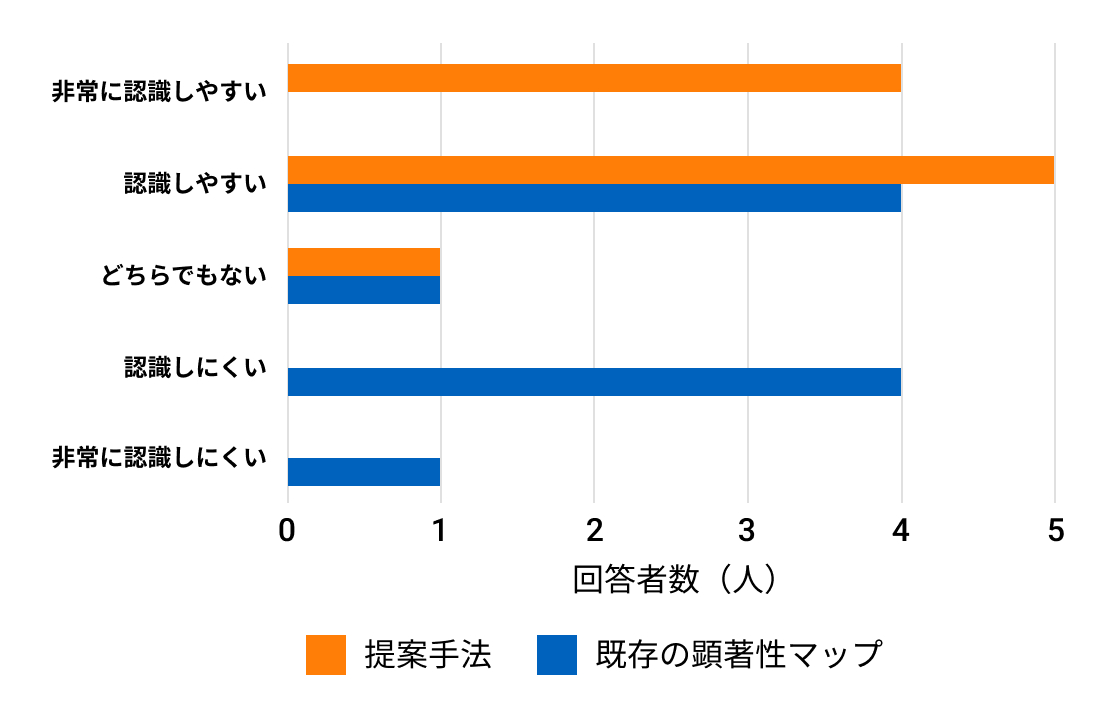
\includegraphics[width=10cm]{figures/07_result01.jpg}
  \caption{顕著領域マップの重要領域の認識のしやすさに関する評価結果}
  \label{fig_evaluation02-1}
\end{figure}

\par また、記述式で質問した既存の顕著性マップと提案手法の顕著領域マップのそれぞれの重要領域の認識のしやすさと認識のしにくさに関する問いでは既存の顕著性マップ重要領域の認識のしずらさとして挙げられた「要素の境界が分かりづらい」や「最も顕著度の高い要素がどれなのか顕著の度合いを比較しにくい」などといった意見を提案手法の顕著領域マップで改善できたという肯定的な意見が多かった。しかしながら様々な意見の中には「元のウェブページの様子が見えない為スクリーンショットと照らし合わせる必要がある」や「顕著度ランキングの枠線の濃淡の差が分かりづらい」などといった元のウェブページの様子が全く見えなくなった提案手法の顕著領域マップならではの問題点もいくつか挙げられた。これらの問題点を解決する為に例えば元のウェブページの画像と顕著領域マップを重ね合わせたり簡単に切り替えることが出来るようなGUIを作成したりランキングの枠の隣に番号を付けるなどの顕著領域マップを作成した後の見せ方にも工夫する必要があることが分かった。上記の提案手法の顕著領域マップの認識のしづらさとして挙げられた問題点は今後の改善に生かして行く必要があると考える。

\par さらに、既存の顕著性マップと提案手法の顕著領域マップのどちらの方が特定の要素の重要度を調べたいときに認識しやすいか質問した問いでは被験者10名全員が提案手法の顕著領域マップの方が優れていると回答した。以上の事から提案手法の顕著領域マップは\ref{subsec:evaluation1}で説明した要素の顕著度推定精度と共に重要領域の認識のしやすさも既存の顕著性マップと比較して改善されたと言える。


\subsubsection{集約図の効果に関する評価}
\par 3つ目の評価方法ではウェブページの特に顕著度が高い要素をランキング順にタイル状に並べて一枚の画像にまとめた集約図の効果について評価した。集約図の効果を測定する為に図\ref{fig_experience03-1}のように集約図の例を見せてウェブページの内容を予想してもらう問いでは「食品系を取り扱う企業のホームページ」などといったざっくりとしたページ内容は被験者全員が理解することが出来た。しかしながら「関東に展開するスーパーを展開する企業」などのより詳細な内容については理解することが難しい結果となった。提案手法の集約図の目的としてこの図を見ることでユーザーが探している内容がウェブページの内容とマッチしているかどうかを一目で確認できるというものがあるが、難しいということが分かった。

\par 顕著度が高い要素を抽出した集約図を見てウェブページの内容をどの程度判断できるかを質問した結果を表\ref{table:evaluation03-1}に示す。被験者の8名が「ある程度判断できる」で2名が「少し判断できる」と回答しており、ほとんどの被験者が集約図を見ることである程度のページの内容を理解することができるということが分かった。次に初見のウェブページの内容を一目で確認したい時に集約図が効果的だと思うかを質問した結果を表\ref{table:evaluation03-2}に示す。こちらの問いでは6名が「効果的である」と答えた一方で「どちらでもない」や「あまり効果的でない」と回答した被験者が2名ずついた。また「非常に効果的である」と回答した被験者がいなかったことから集約図を閲覧することでウェブページの大枠は理解できるものの細かい内容についてまでは理解できないということが確認できた。集約図のウェブページの内容を一目で確認するという目的については現状では達成できておらず、表示項目を増やしたりレイアウトや見せ方を変更するなどの工夫が必要であることが分かった。

\begin{table}[H]
    \caption{Q8の回答結果}
    \label{table:evaluation03-1}
    \centering
    \begin{tabular}{lc}
      \hline
      選択肢 & 回答数 \\
      \hline \hline
      ある程度判断できる & 8 \\
      ほとんど判断できる & 0 \\
      少し判断できる & 2 \\
      全く判断できない & 0 \\
      \hline
    \end{tabular}
\end{table}

\begin{table}[H]
    \caption{Q9の回答結果}
    \label{table:evaluation03-2}
    \centering
    \begin{tabular}{lc}
      \hline
      選択肢 & 回答数 \\
      \hline \hline
      非常に効果的である & 0 \\
      効果的である & 6 \\
      どちらでもない & 2 \\
      あまり効果的でない & 2 \\
      全く効果的でない & 0 \\
      \hline
    \end{tabular}
\end{table}
